\documentclass[a4page,notitlepage]{article}
\usepackage{color,soul,amsmath,graphicx}
\usepackage[outercaption]{sidecap}
\usepackage[citestyle=authoryear]{biblatex}
\usepackage[font=small,labelfont=bf]{caption}
\sidecaptionvpos{figure}{c}
\providecommand{\abs}[1]{\lvert#1\rvert}
\providecommand{\norm}[1]{\lVert#1\rVert}

\title{Analyzing stability of very simple metabolic cycles}
\author{Uri Barenholz}
\date{August 2013}

\begin{document}
\abstract{
    Auto-catalytic cycles are an important part of metabolic networks.
    As the flux in auto-catalytic cycles both depends on the concentration of intermediate metabolites, and affects it, they present unique features and characteristics.
    An understanding of the constraints under which metabolic auto-catalytic cycles operate is essential both for understaning limitations of existing metabolic networks, and to successfully modify them in synthetic biology metabolic engineering applications.

    We analyze two simple metabolic auto-catalytic cycles, presenting the mathematical tools and techniques needed in order to gain insights about their operation.
    We show that even for very simple cycles, specific constraints on the kinetic parameters of the enzymes are needed in order to allow a stable flux through the cycle.
    This work thus serves as an approachable introduction to the analysis of auto-catalytic metabolic cycles and to derive specific insights about the cycles we analyze.
}

\section{Introduction}

    This document describes the dynamic analysis of a carbon fixating auto-catalytic cycle (Figure \ref{fig:autocatal}). The result of the analysis reveals that such an auto-catalytic cycle always has a steady state point when the concentrations along the cycle are all 0, and under some conditions may have another steady state point at a positive concentration.
    Furhtermore, the conclusion of the analysis is that, in case two steady state points exists (at 0 and $C$), then the relation between $\frac{V_{\max,b}}{K_{m,b}}$ and $\frac{V_{\max,a}}{K_{m,a}}$, (where $V_{\max,b},K_{m,b}$ are the Michaelis-Menten parameters of the biomass reaction and $V_{\max,a},K_{m,a}$ are the parameters of the carbon-fixating auto-catalytic reaction) determine which of the two steady state points is stable.
    If $\frac{V_{\max,b}}{K_{m,b}} > \frac{V_{\max,a}}{K_{m,a}}$ then 0 is the stable steady state, and if $\frac{V_{\max,b}}{K_{m,b}} < \frac{V_{\max,a}}{K_{m,a}}$ then the non-zero point is the stable steady state of the system.
\section{Introduction}
\begin{figure}[h]
\centering
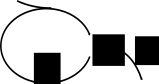
\includegraphics{cycle3.pdf}
\caption{A simple auto-catalytic cycle with extration of biomass reaction}
\label{fig:autocatal}
\end{figure}
Biological systems are noisy by nature.
Thus, in order for metabolic pathways and cycles to be viable, they must be resistant to noise (meaning they should be able to perform their action, maintaining fluxes and concentrations, where necessary, even under perturbations).

We define a metabolic equilibrium state as a state where the concentrations of intermediate metabolites remains constant (excluding external input and output reactions, as defined by the topology of the network and problem at hand).
We will be investigating the number of equilibrium points, their respective concentrations and fluxes, and their stability.
By stability we refer to the ability of a network to converge back to the same equilibrium point in cases of small perturbations around it.

Mathematically we will be working in a vector space of the concentrations of the different metabolites, such that if there are two metabolites, $M_1$ and $M_2$, then $\vec{C}=(C_1,C_2)$ represents the state where $M_1$'s concentration is $C_1$ and $M_2$'s concentration is $C_2$.
If we now define a vectoric flux function, $\frac{d\vec{C}}{dt}=\vec{F}(\vec{C})$ (that is, a function that takes a vector of concentrations and returns the time derivative of each of the concentrations as a result of the implied network fluxes), we can formally define an equilibrium point, $\vec{C}^*$ as any point for which: $\vec{F}(\vec{C}^*)=0$.
Furthermore - dynamic theory states that such an equilibrium point will be stable iff the real parts of the eigenvalues of the Jacobian matrix of $\vec{F}()$ at $\vec{C}^*$ are all negative.

\section{Analyzing a simple cycle}
To warm up and get comfortable with the analysis method, we start with the simplest metabolic cycle possible, as is depicted in Figure \ref{simple-cycle}.
\begin{figure}[h]
\centering
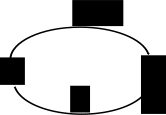
\includegraphics{cycle1.pdf}
\caption{A simple metabolic cycle}
\label{simple-cycle}
\end{figure}
For simplicity we will assume that $V_1$ is only a function of $C_1$, and $V_2$ is only a function of $C_2$.
Thus we get that:
\[\frac{d\vec{C}}{dt}=\vec{F}(C_1,C_2) = \bigg(
\begin{matrix}
    V_2(C_2)-V_1(C_1) \\
    V_1(C_1)-V_2(C_2)
\end{matrix}
\bigg)\]
Therefore an equilibrium point $\vec{C}^*$ must satisfy that: $\vec{F}(\vec{C}^*)=0$ implying that $V_1(C_1^*)=V_2(C_2^*)$.
In order to analyze stability we need to calculate the Jacobian matrix of $\vec{F}()$ which (once noting that $\frac{dV_1}{dC_2}=\frac{dV_2}{dC_1}=0$) becomes:
\[
J=\bigg(
\begin{matrix}
    -\frac{dV_1}{dC_1} & \frac{dV_2}{dC_2} \\
    \frac{dV_1}{dC_1} & -\frac{dV_2}{dC_2}
\end{matrix}
\bigg)
\]
If we use the notation of: $k_1=\frac{dV_1}{dC_1}$ and $k_2=\frac{dV_2}{dC_2}$, we can write the characteristic polynomial of the Jacobian matrix (the roots of which are its eigenvalues) as:
\[
\text{det}(\lambda I -J)=(\lambda+k_1)(\lambda+k_2)-k_1k_2=\lambda^2+(k_1+k_2)\lambda
\]
Which immediately indicates that the eigen values are $0$ and $-(k_1+k_2)$.
We can therefore conclude that no equilibrium point is stable, as all will have at least one non-negative eigenvalue.
However, if $k_1+k_2$ is positive, then the equilibrium point is semi-stable, in the sense that there is some direction (the direction corresponding to the eigen-vector with the $0$ eigenvalue) that is tangent to a line of equilibrium points (so small perturbations along this line will keep the system at equilibrium, but not the same equilibrium), and perturbations in the direction of the other eigenvector will return to the same equilibrium point.
Furthermore - as this setup, being a closed cycle, possesses the specific feature of conservation of mass (mathematically - $C_1+C_2$ is constant in time), and as each equilibrium point $\vec{C^*}$ can be characterized by such a total mass, if the perturbations do not change the total mass, the system will converge to the same equilibrium point, and if they do change the total mass, the system will converge to the unique equilibrium point defined for the modified mass.

As a sidenote, we coment that for Michaelis-Menten (MM) dynamics the derivatives are always positive, so that case results in all equilibrium points being semi-stable and conform to the analysis above.
\section{Analyzing a simple open cycle}
Once we got a little bit of a feel for the analysis of the dynamics of simple metabolic networks, we turn to a slightly more complicated case, as is depicted in Figure \ref{open-cycle}.
\begin{figure}[h]
\centering
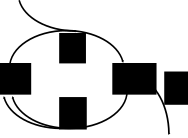
\includegraphics{cycle2.pdf}
\caption{A simple open metabolic cycle}
\label{open-cycle}
\end{figure}
Here the flux function is:
\[
\frac{d\vec{C}}{dt}=\vec{F}(\vec{C})=
\bigg(
\begin{matrix}
2V_2(C_2)-V_1(C_1) \\
V_1(C_1)-V_2(C_2)-V_3(C_2)
\end{matrix}
\bigg)
\]
Therefore equilibrium points must satisfy (for $C_1*$) that:
\[
2V_2(C_2^*)-V_1(C_1^*)=0 \rightarrow V_2(C_2^*)=V_1(C_1^*)/2
\]
and for $C_2^*$ (when substituting the above):
\[
V_1(C_1^*)-V_2(C_2^*)-V_3(C_2^*)=0 \rightarrow V_2(C_2^*)-V_3(C_2^*)=0 \rightarrow V_2(C_2^*)=V_3(C_2^*)
\]
So an equilibrium point must satisfy that:
\[ V_1(C_1^*)/2=V_2(C_2^*)=V_3(C_2^*) \]
For the current analysis we will consider two types of kinetics for $V_1$, $V_2$ and $V_3$: Linear and simple Michaelis-Menten.
We note that fluxes are alway zero when the substrate concentration is zero, implying that linear kinetics must be of the form $V(C)=aC$, and that the fluxes always increase when the substrate concentration increases, implying that the flux derivative w.r.t. its substrate is always positive.
Using the same notation as in the previous section for $k_1$, $k_2$ and $k_3$, we can write the Jacobian matrix of $V$ as:
\[
J=\bigg(
\begin{matrix}
    -k_1 & 2k_2 \\
    k_1 & -k_2-k_3
\end{matrix}
\bigg)
\]
and the characteristic polynomial is thus:
\[
\text{det}(\lambda I -J)=(\lambda+k_1)(\lambda+k_2+k_3)-2k_1k_2=\lambda^2+(k_1+k_2+k_3)\lambda -k_1k_2+k_1k_3
\]
The eigenvalues are therefore:
\[
\lambda_{1,2}=\frac{-(k_1+k_2+k_3)\pm \sqrt{(k_1+k_2+k_3)^2+4k_1k_2-4k_1k_3}}{2}
\]
Therefore, in order for the real part of both eigenvalues to be negative (the condition for a stable equilibrium point), $k_1+k_2+k_3$ must be positive (which always holds as $k_i>0$ for all $i$) and $4k_1k_2-4k_1k_3$ must be negative (implying that $k_3>k_2$, given that $k_1$ is positive).

We now turn to see what possible combinations of kinetics can satisfy these conditions:
\begin{itemize}
\item We note that the case of both $V_2$ and $V_3$ being linear (meaning that $V_2(C_2)=a_2C_2;V_3(C_2)=a_3C_2)$ is unprobable as it requires that $a_2=a_3$ in order for an equilibrium point to exist.
\item If $V_2$ is linear and $V_3$ is MM, then they must intersect at an equilibrium point.
They intersect at the trivial point where $C_2=0$.
As MM is a concave function, if they intersect at a larger concentration point, then at the point of intersection $k_3$ will be smaller than $a_2=k_2$ making that point unstable.
\end{itemize}
We therefore conclude that $V_2$ cannot be linear but rather must be MM, and that $V_1$ and $V_3$ can be either linear or MM.

As at an equilibrium point $V_2(C_2^*)=V_3(C_2^*)$, and as we are restricted to linear or MM kinetics, it follows that there is at most only one concentration $C_2$ (other than $C_2=0$) for which this condition holds.
For this concentration, if there exists a concentration $C_1$ that satisfies $V_1(C_1)/2=V_2(C_2)$ then there exists an equilibrium point for the metabolic network.
At these concentrations, if $k_3>k_2$ (as is always the case for linear $V_3$, and is sometimes the case for MM $k_2,k_3$, which we will analyze below), then the equilibrium point is stable.

To get some intuition on how stability works, if we assume that the system is in the equilibrium state, and then somehow a small deviation in the concentrations occure - then there are two possibilities: either the total number of carbons in the cycle ($C_1+C_2$) increased, or it decreased.
If it increased - then at some point $C_2$'s concentration will be above the equilibrium point.
At this point - as $k_3>k_2$, more carbons will be taken out of the cycle via $V_3$ than recycled via $V_2$, thus decreasing the total number of carbons in the cycle.
If, on the other hand, the total number of carbons in the cycle is somewhat smaller than the number at the equilibrium state, then at some point $C_2$ will be smaller than its value at the equilibrium point, resulting in $V_2>V_3$.
At this point, the flux of carbons out of the cycle is smaller than the flux of carbons that are recycled in the cycle.
As new carbons are being added to the cycle via $V_1$, the total number of carbons in the cycle will increase.

\subsection{Analyzing intersection points of MM kinetics and linear kinetics}
The general form of a MM kinetics equation is:
\[
V(C)=\frac{V_{max}C}{K_m+C}
\]
Therefore, it intersects a straight line of the form $V(C)=aC$ at the solutions to the equation:
\[
aC=\frac{V_{max}C}{K_m+C} \rightarrow aC^2+C(aK_m-V_{max})
\]
that is, at $C=0$ and $C=V_{max}-aK_m$
In order for the non-trivial solution to be feasible we must therefore require that $V_{max}>aK_m$.

In the case of two MM kinetics fluxes:
\[
V_a(C)=\frac{V_{a,max}C}{K_{a,m}+C};
V_b(C)=\frac{V_{b,max}C}{K_{b,m}+C}
\]
The intersection points are the solutions to the equation:
\[
\frac{V_{a,max}C}{K_{a,m}+C}=\frac{V_{b,max}C}{K_{b,m}+C} \rightarrow (V_{a,max}C)(K_{b,m}+C)=(V_{b,max}C)(K_{a,m}+C)
\]
Which are at $C=0$ and at:
\[
C(V_{a,max}-V_{b,max})=V_{b,max}K_{a,m}-V_{a,max}K_{b,m} \rightarrow C=\frac{V_{b,max}K_{a,m}-V_{a,max}K_{b,m}}{V_{a,max}-V_{b,max}}
\]
Requiring a positive intersection and assuming w.l.o.g. that $V_{a,max}>V_{b,max}$ thus gives:
\[
V_{b,max}K_{a,m}-V_{a,max}K_{b,m}>0 \rightarrow V_{b,max}K_{a,m}>V_{a,max}K_{b,m}
\]
concluding that:
\[
\frac{V_{b,max}}{V_{a,max}}>\frac{K_{b,m}}{K_{a,m}}
\]
Integrating this result with the stability requirement (that at the intersection point $k_3>k_2$), noting that this implies that $V_{3,max}>V_{2,max}$ we must therefore assign $a \rightarrow 3$ and $b \rightarrow 2$ to get:
\[
\frac{V_{2,max}}{V_{3,max}}>\frac{K_{2,m}}{K_{3,m}}
\]
as the requirement on the kinetic parameters of $V_2()$ and $V_3()$.

TODO: add analysis of convergence via analytical solution to linear differential equations.
analyze cases of substrate inhibition.
\end{document}
